\documentclass[11pt]{amsart}
\usepackage[T1]{fontenc}
\usepackage{lmodern}
\usepackage{microtype}
\usepackage{booktabs}
\usepackage{tikz}
\usepackage[hidelinks]{hyperref}
\newtheorem{theorem}{Theorem}
\newtheorem{lemma}[theorem]{Lemma}
\newcommand{\up}{\mathrel{\nearrow}}
\newcommand{\moveup}{\(2\)--\(3\)}
\newcommand{\movedown}{\(3\)--\(2\)}
\newcommand{\twotozero}{\(2\)--\(0\)}
\newcommand{\zerototwo}{\(0\)--\(2\)}
\title{Unimodal Pachner paths for three-manifold triangulations}
\author{Kaiwen Jin}
\email{yui.ui.siki@gmail.com}
\subjclass[2020]{57Q15, 57K99}
\keywords{Pachner moves, generalized triangulations, special spines}
\begin{document}
\begin{abstract}
Let \(M\) be a compact connected \(3\)-manifold with no spherical
boundary components. We prove that any two generalized triangulations of
\(M\) in the closed case, or ideal triangulations when the boundary is nonempty, have
a common descendant by \(2\)--\(3\) Pachner moves whenever they have the same
number of internal vertices and at least two tetrahedra each. This gives the
unimodal sequence of \(2\)--\(3\) and \(3\)--\(2\) moves conjectured by Burton
and He. Their arch construction reduces the question to a comparison of a
triangulation and an enlargement along a marked path in its dual spine. We use
the noncrossing order of the path arcs in a spine face to shorten an arch by
positive moves on both sides of this comparison.
\end{abstract}
\maketitle

\section{Introduction}

A \moveup\ Pachner move retriangulates two tetrahedra that meet along a
triangle as three around an edge. The Matveev--Piergallini calculus and its
extension to ideal triangulations connect triangulations by these moves and
their inverses, subject to the vertex count and the one-tetrahedron
exception \cite{amendola,rst}. Burton and He asked whether these paths can be
chosen to have a single maximum in the tetrahedron count, with all
\moveup\ moves preceding all \movedown\ moves \cite[Conjecture~8]{bh}. Their
Theorem~9 gives a unimodal path with \twotozero\ moves in the descending
part. The descending moves in the conjecture are the inverses of the
ascending moves, so this is also a question about common descendants under
\moveup\ moves.

\begin{theorem}\label{thm:main}
Let \(M\) be a compact connected \(3\)-manifold with no \(2\)-sphere boundary
components. Let \(T,U\) be generalized triangulations of \(M\) if \(M\) is
closed, or ideal triangulations representing \(M\) otherwise. Thus the facets
of finitely many tetrahedra are affinely paired, and no edge is identified
with itself in reverse. A vertex with a \(2\)-sphere link is internal, and
truncating all other vertices gives the boundary of \(M\). Suppose each
triangulation has at least two tetrahedra and the two have the same number
of internal vertices. Then \(T\) and \(U\) have a common descendant by finite
sequences of legal \(2\)--\(3\) moves, either of which may be empty.
\end{theorem}

The proof uses the arch of Burton and He to copy a \movedown\ move and
subsequent \moveup\ moves on an enlarged triangulation. Removing the arch
amounts to joining two triangulations by \moveup\ moves. The new step is to
shorten the arch along an arc in an edge-link disk. After preparing the edge
occurrences, the base uses two moves and the enlarged triangulation uses one.
The same operation can then be applied to the shorter arch.

\section{Local moves and the marked arch}\label{sec:arch}

Write \(X\up Y\) if \(Y\) can be reached from \(X\) by finitely many
\moveup\ moves, including the empty sequence. Equality of endpoints means
combinatorial isomorphism with the affine face pairings.

The arbitrary-order connectivity theorem applies in the conventions of
\cite[Notation~6 and Theorem~7]{bh}. To obtain this formulation from
\cite[Corollary~2.2]{amendola}, take the arc marking empty and delete a small
ball at each internal vertex. The number of these punctures is the same for
the two triangulations, and their fully truncated manifolds are
homeomorphic. The two loose ideal triangulations are connected by
Matveev--Piergallini moves. These preserve the vertex links, so the spherical
boundary components can again be filled. See also \cite[Theorem~1.4]{rst}.

In a finite mixed path, keep a prefix followed by a suffix of \movedown\
moves, initially empty. Take the last \movedown\ move in the prefix, if
there is one, and the positive tail following it in the prefix. Let \(P,Q\)
be the ends of this segment. If \(P\up Z\) and \(Q\up Z\), use the former
path and put the inverse of the latter in front of the old suffix. The
number of \movedown\ moves in the prefix decreases by one. Thus it suffices
to join \(P,Q\) whenever one \movedown\ move and then a finite positive
sequence lead from \(P\) to \(Q\).

\subsection{Relative replacements}

In a \moveup\ move, keep the chosen common facet of the two distinct
tetrahedra and open all six exterior facets. The resulting bipyramid has
two triangulations with identical boundary triangles. Retriangulating it
and restoring all exterior affine maps preserves the quotient, even if
some of the exterior facets are paired to one another or the corner
images coincide. It preserves vertex links because the triangulations
of the same ball have the same boundary vertices and agree on the
boundary. Each old edge of the support is on its boundary. Its occurrences
and endpoint identifications transport through those triangles. The new
diagonal is interior, with a cyclic link and consistent endpoint labels.
In particular no edge becomes reversed, and truncation preserves the
represented manifold. The same reasoning applies to a word in the
bipyramid. Use an internal pairing between distinct tetrahedra at each step and carry forward the same
six exterior triangle occurrences with their affine coordinates. Restoring
any admissible exterior gluings then gives the same word in the quotient.

For an edge class \(e\) of a generalized triangulation, the cyclic link
records a corner for each local tetrahedral edge representing \(e\), and
a side for each triangular face incidence at \(e\). We fill this circle
with a disk, the characteristic disk of the dual spine face. Its
boundary records occurrences even if some are identified in the spine.
A paired triangular face contributes a side for each of its three edges,
possibly several in one disk. Each side carries the interval between the
two half-facets in their link order.

\subsection{Marking and lifting a path}

Choose finitely many distinct points, called buttresses, in the interiors of
the paired-face intervals. A buttress on a triangle \(cuv\) selects the
corner \(c\), giving endpoints on the two disk sides for \(cu,cv\).
For example, if the two half-facets belong to \(A\) and \(B\), the mark
appears between the corresponding \(A\) and \(B\) corners on each disk
side. Connect endpoints by disjoint piecewise-linear chords in the disks,
with two terminal arcs from boundary points to interior points, so the
arcs and buttresses form a single path. Require the two \(c\) labels at
the ends of each chord to represent the same end of its edge after
following the affine identifications in the link. If a chord joins the
\(cu\) slot to a slot of another marked face, each side of that chord
meets one half-facet of each face, and so specifies their correspondence. This is the marked data of a
wall in the terminology of \cite[Section~3.1]{bh}. We will construct it directly.

In the lift, keep all tetrahedra of the base, calling them natural
tetrahedra. Insert into every marked pairing a chain of tetrahedra in
the order of its buttresses. The tetrahedron of a buttress at \(cuv\) is
\[
                 S=(c_0,c_1,u,v).
\]
Its faces \(c_0uv,c_1uv\) give the two sides of the subdivision in the
chain, using the old face coordinates. Its faces \(c_0c_1u,c_0c_1v\)
are attached along the corresponding path arcs. Along a chord identify
the two doubled corners by matching the sides of the chord and pair the
third corners to each other. At the two terminal arcs attach the cap
\((c_0,c_1,u_0,u_r)\) on \(c_0c_1u_0\) and \(c_0c_1u_r\), matching the
nondoubled end of each terminal edge to its \(u_i\), for \(i=0,r\),
where \(r\) is the number of buttresses. Fix the first
attachment's \(c_0,c_1\) labels and use their transport along the
subdivision chain to label the other attachment. This determines the cap
maps up to relabelling the cap's two \(c\) corners simultaneously. Its
other two facets pair by swapping \(c_0,c_1\) and fixing \(u_0,u_r\).
The cap and the chain of subdivisions form the arch. In any legal lift the
link of the doubled edge has these cells as its occurrences, with no
reversal around the link.

Here is the seed for copying a \movedown\ move, in the relative chart of
\cite[Fig.~16]{bh}. Use input cells \(abxy,abxz,D=abyz\) around the
edge \(ab\), writing the local corner names together to denote a cell
or facet. The \movedown\ output comprises \(axyz,bxyz\) joined on \(xyz\).
Instead, apply \moveup\ to the pair across \(abx\). This gives the cells
\(axyz,bxyz\) and \(C=abyz\), with the untouched cell \(D\) paired to \(C\)
across \(aby\) and \(abz\). Apply \moveup\ at \(aby\) between \(C,D\),
with apices \(z_0,z_1\) from \(C,D\). The new cells are
\[
                (a,y,z_0,z_1),\quad (b,y,z_0,z_1),\quad (a,b,z_0,z_1).
\]
The first two attach to \(axyz,bxyz\) at \(ayz_0,byz_0\) and to the
former exterior faces of \(D\) at \(ayz_1,byz_1\), respectively. They
are joined on \(yz_0z_1\) and attach to the cap on \(az_0z_1,bz_0z_1\).
The former \(abz\) pairing folds the two remaining facets of the cap.
All six old exterior maps have their specified affine coordinates.

In the base put a buttress selecting \(z\) at each of \(ayz,byz\), close
to the half in the natural cell. The chord in the \(yz\) disk follows the
boundary interval through the two natural cells across \(xyz\). Its
same-side match is \(z_0\) to \(z_0\) on the side of this interval. The
two terminal arcs in the \(az,bz\) disks can be chosen close to their
endpoints. Even if exterior gluing identifies the two marked faces, the
prescribed positions are near the opposite ends of their common interval.
The two incidence corners of the chord interval are distinct, and all
terminal positions are other incidences or different positions on a repeated
side. This constructs disjoint arcs with the required matches for arbitrary
exterior affine pairings.

\subsection{Copying an increasing move}

Call a paired face free if it has no buttress. A \moveup\ move at a free
pairing can be done both in the base and in the lift on the same natural
cells. In each old edge link it replaces intervals of corners and sides
inside the bipyramid, with the same ends at the exterior. All marked
positions and their half-facet sides transport in order. The three new
internal pairings are free.

A mark blocking such a move can be slid off the face through a natural
tetrahedron. Suppose \(A=(c_0,u,v,d)\) is at one end of the subdivision
chain of \(cuv\), and \(S=(c_0,c_1,u,v)\) is the closest subdivision.
The \moveup\ move on \(c_0uv\) gives
\[
          A'=(c_1,u,v,d),\qquad (c_0,c_1,u,d),\qquad (c_0,c_1,v,d).
\]
The first cell is natural in the original coordinates, with \(c_1\)
as its \(c\). Its \(c_1uv\) joins the remaining chain. The other two
cells subdivide the exterior pairings on \(cud,cvd\), with a shared
facet \(c_0c_1d\). Each joins \(A'\) on the facet with \(c_1\) alone,
and the old opposite half of the exterior pairing on the facet with
\(c_0\) alone. They inherit the attachments along \(c_0c_1u,c_0c_1v\)
from \(S\). In the \(cu,cv\) disks slide the two endpoints
along the boundary past the respective corner of \(A\), into the
adjoining end gaps. The intervals are clear because the first buttress
from \(A\) was chosen. The side towards \(A\) before the slide is the
forward side of this boundary motion. At the new endpoints it faces
away from \(A'\) and retains \(c_0\). Join the two new endpoints in the
\(cd\) disk by a short arc at its \(A\) corner. Both near halves there
carry \(c_1\), giving the displayed matching. All three corners are
distinct as occurrences, even if some edge classes agree. These boundary
motions stay in the end gaps of their sides, including when another
facet of \(A\) belongs to the same paired face. The new chord and the
moved endpoints can thus be put in the indicated collars without
intersecting the other arcs.

The slide uses only positive moves on the lift, as in
\cite[Lemma~11]{bh}. At a marked pairing between distinct natural cells
one can repeatedly slide from one end until the pairing is free, then
copy the move. It is also possible to send any prefix of the chain
towards one end and the remaining subdivisions towards the other.
Starting from the seed, perform this copying along the positive tail
of the segment from \(P\) to \(Q\). This reaches \(Q\) with a marked
arch. It remains to join this lift and the base.

\section{Separating repeated incidences}\label{sec:normalize}

The free face pairings give a graph whose vertices are the natural
tetrahedra. A loop does not give a distinct neighbour. If a vertex
\(A\) is isolated from all other vertices in this graph, take a marked
face joining \(A\) to a distinct \(B\), which exists by connectedness
of the full face-pairing graph and the presence of at least two cells.
Slide its whole chain toward \(A\) and copy a \moveup\ move at the
cleared face. Any newly marked exterior pairing was incident to \(A\)
and provided no free distinct neighbour. The three new cells are
joined by their free internal triangle of adjacencies. Every previous
free adjacency to a distinct cell, other than those between removed
cells, still has its exterior pairing carried to a new cell. Thus the
number of singleton free components decreases. After finitely many
steps every cell has a free pairing to a distinct cell. Copying other
free moves preserves this property.

\begin{lemma}\label{lem:separate}
Fix the edge classes of the current base. Suppose its free pairing graph
has no singleton component. Copied positive moves can arrange that each
marked half-facet has its own cell. Call these cells protected. Any cell
with two or more occurrences of fixed edge classes has all of them
on its protected facet. There is no free pairing between protected
cells, including a loop. Each unprotected cell has a distinct
unprotected free neighbour.
\end{lemma}
\begin{proof}
Use the bipyramid replacement of Appendix~\ref{sec:certs}. It puts
the six outer facets in different cells, with no internal pairing
between two outer-facet cells. Each cell has an internal pairing
with a distinct cell that carries no outer facet. Each new cell with
two or more occurrences of bipyramid boundary edges has them all on
its one outer facet, and an internal face has at most one such
occurrence.

Apply the replacement at every original free face, carrying the
remaining faces through the unchanged outer facets. To process a
self-pairing, first use a free adjacency of its carrier to a distinct
cell. This replacement separates the two halves of the self-pairing.
The interior graph of each replacement is connected, since each
successive \moveup\ step replaces two vertices by an internally
connected triple. Thus the free graph keeps its no-singleton
property. The procedure is finite since it processes a fixed list,
and an auxiliary replacement used at another original free face
processes that face as well.

At the end, each cell was created by a replacement, since each old
cell was incident to at least one of the original free pairings.
Its only possible outer facet from the original triangulation is a
marked half-facet. A fixed edge class in the latest replacement
containing this cell must come from a boundary edge of that
bipyramid. If the cell has an outer facet from a previous
replacement's interior, that facet could carry at most one fixed
edge occurrence. The bipyramid properties give the claimed counts.
A free pairing of protected cells created in the same replacement
would join two outer-facet cells internally. For cells created at
different times, it would require a second outer facet of the newer
cell. Finally an unprotected surviving cell has a distinct neighbour
without an outer facet in the replacement that created it. Their shared
free face cannot be consumed while the surviving cell stays in place.
If the neighbouring cell is subsequently replaced, the shared face is
the only outer facet of its new carrier, which is still unprotected.
\end{proof}

When a face has \(k\ge 2\) buttresses, apply Lemma~\ref{lem:separate}.
The two natural cells at that face have six distinct free exterior
pairings to unprotected neighbours. Slide one buttress through one
end and the other \(k-1\) through the other and copy a move at the
cleared face. Each of the six exterior pairings gets at most \(k-1\)
buttresses. The other counts are unchanged. The remaining unprotected
cells still have unprotected neighbours, and the remaining protected
cells had no free pairing to either removed cell. The three new
cells have free pairings with one another. Hence there is still no
singleton. The vector counting pairings of each multiplicity
\(\ge 2\), starting at the original maximum and reading downwards,
decreases lexicographically. After finitely many repetitions the
marked faces have one buttress each.

We next ensure that in each marked triangle the two edge classes used
by its buttress are different, and that the third edge belongs to no
class used by any buttress. For a marked triangle \(cxy\), apply
Lemma~\ref{lem:separate} with all the current edge classes fixed. Choose
one of its natural ends \(A=(c,x,y,d)\). The opposite face \(xyd\)
is free, paired to a distinct unprotected cell \(B=(z,x,y,d)\). This
cell contains the fixed edge \(xy\). Lemma~\ref{lem:separate} bounds an
unprotected cell by one fixed-edge occurrence, so \(xz\) and \(yz\)
in \(B\) are outside the fixed set. Copy the move on \(xyd\). Along
the new diagonal \(cz\) are three cells
\[
               (c,z,x,y),\qquad (c,z,x,d),\qquad (c,z,y,d).
\]
Slide the buttress on \(cxy\) towards the first cell and copy the
move on \(cxy\). The two new buttresses lie at \(czx,czy\) on what were
internal pairings of the first move. The used edge sequence is now
\(cx,cz,cy\) and the third edges of the two new triangles are \(xz,yz\).
The two other cells of the first move still meet on the free face
\(czd\), the three cells of the last move are freely adjacent, and
other cells have lost no free pairings. This keeps the no-singleton
property. The new label \(cz\) was just created and occurs only once
in the path. Subsequent applications insert only newly created labels
and cannot turn a previously unused third edge into a path label.
Apply the operation once at each of the pre-existing marked faces.
This proves the required incidence condition, and also gives a way
to restore it at an individual defective mark later.

\section{Shortening the arch}\label{sec:shorten}

Suppose there is a chord in the disk for a used edge \(e\).
Among the chords in this disk there is one with a complementary
boundary interval containing no other chord endpoint and at most one
terminal endpoint. Indeed the endpoints of two chords cannot
alternate. Start with the two open boundary intervals of any chord.
An interval that meets other chord endpoints contains a complete pair.
Replace such an interval by
an inclusion-minimal closed interval between paired endpoints in it,
and take the interior. In this way both initial sides give intervals
with disjoint interiors free of chord endpoints. There are at most two
terminal endpoints in total, so at least one of the two has at most one.
Figure~\ref{fig:ear} shows the case with a terminal endpoint on the
selected side.

\begin{figure}[ht]
\centering
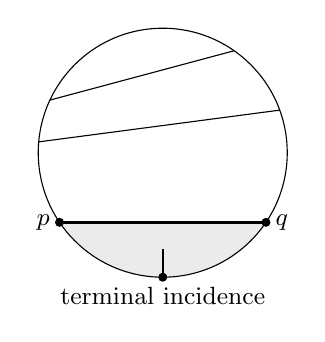
\begin{tikzpicture}[scale=1.02,every node/.style={font=\small}]
  \coordinate (p) at (214:1.55);
  \coordinate (q) at (326:1.55);
  \coordinate (t) at (270:1.55);
  \fill[black!8] (p) arc[start angle=214,end angle=326,radius=1.55] -- cycle;
  \draw (0,0) circle (1.55);
  \draw[very thick] (p) -- (q);
  \draw (155:1.55) -- (55:1.55);
  \draw (175:1.55) -- (20:1.55);
  \draw[semithick] (t) -- (0,-1.2);
  \foreach \v in {p,q,t} \fill (\v) circle (1.6pt);
  \node[left] at (p) {\(p\)};
  \node[right] at (q) {\(q\)};
  \node[below] at (t) {terminal incidence};
\end{tikzpicture}
\caption{A chord in an edge-link disk. The shaded side meets at most one
terminal arc. Its boundary interval determines the two cuts of the base
replacement.}
\label{fig:ear}
\end{figure}

Let \(p,q\) be the two end faces of the selected chord. The incidence
condition implies that each marked face meets the circle for \(e\) at
most once, only at a used slot. Thus \(p,q\) are distinct, and the
selected link interval has no further mark except possibly the terminal
one. Apply Lemma~\ref{lem:separate} relative to the current edges.
Every natural cell around \(e\) has a single occurrence of \(e\).
The endpoint half-facets are carried by different cells. Two adjacent
cells in the interval meeting on a free triangle containing \(e\) can
be compressed into one cell about \(e\) by a copied \moveup\ move. In
the bipyramid the unique new tetrahedron whose vertices include both
ends of the local \(e\) has the two outer triangles through \(e\).
The others have no occurrence of it, because the input cells had
only the specified occurrence and new diagonals are interior. Compress
until the interval contains two cells. If it has an interior terminal
pairing, compress until one cell remains on each side of it.

Use occurrence labels \(cxuv,cxwv\) for the two cells, sharing \(cxv\),
with \(e=cx\), \(p=cxu\), and \(q=cxw\). Denote the halves of \(p,q\)
in these two cells by \(p_{\mathrm{in}},q_{\mathrm{in}}\) and their
opposite halves by \(p_{\mathrm{out}},q_{\mathrm{out}}\).
\begin{itemize}
\item In the base, move at \(cxv\), creating \(cxuw,cvuw,xvuw\).
  Then move at \(vuw\) between the latter two cells. The outputs are
  the two original natural cells, again meeting at \(cxv\), and two
  pillows \(cxuw\). The inner pillow attaches to \(p_{\mathrm{in}}\)
  on \(cxu\) and \(q_{\mathrm{in}}\) on \(cxw\). The outer attaches to
  \(p_{\mathrm{out}},q_{\mathrm{out}}\) on the corresponding faces.
  The pillows share \(cuw\) and \(xuw\). This gives a two-cell
  \zerototwo\ insertion by two \moveup\ moves \cite[Fig.~28]{amendola}.
  Every exterior map and the pairing at the original seam \(cxv\)
  have their original affine coordinates.
\item In the lift, the subdivisions \((c_0,c_1,x,u)\) and
  \((c_0,c_1,x,w)\) meet on \(c_0c_1x\). On both subdivisions choose
  \(c_0\) on the side of the chord facing the selected interval. Apply
  \moveup\ at their common facet to get
  \[
          (c_0,x,u,w),\qquad(c_1,x,u,w),\qquad(c_0,c_1,u,w).
  \]
  The first two meet at \(xuw\) and join opposite sides of the
  third on the faces \(c_suw\). The \(c_0\) cell retains the original
  attachments to \(p_{\mathrm{in}},q_{\mathrm{in}}\). The \(c_1\) cell
  retains those to \(p_{\mathrm{out}},q_{\mathrm{out}}\). The third
  cell inherits the attachments at \(c_0c_1u,c_0c_1w\).
  The first two cells are exactly the two base pillows, with the
  third a new subdivision at their common face \(cuw\).
\end{itemize}
The possible terminal mark on \(cxv\) stays where it was in the lift.
The moves in the base use this face during the replacement and restore
its pairing at the end. Thus the two paths advance to a base and its
lift with one fewer buttress.

The \(cx\) edge of the outer pillow already existed after the first
move. Its link is the complementary \(p\)-to-\(q\) interval closed by
the outer pillow corner and includes the old exterior identifications.
The \(cx\) in the inner pillow is the new diagonal of the second move.
Its link is the selected interval, including the preserved seam \(cxv\),
closed by the inner pillow corner. This diagonal does not meet the
exterior, so the two copies cannot be identified by regluing.

Cut the old \(e\) disk along the removed chord. The two resulting disks
have the respective old \(p\)-to-\(q\) intervals and one new pillow
corner each on their boundaries. Every other arc of the old disk is
in one piece with its previous boundary positions and orientation.
In the \(cu\) link the old
crossing of \(p\) is extended through the two pillows, with \(cuw\) as
the middle face. Similarly the \(cw\) link extends the crossing of
\(q\). These carry the two unused chord or terminal attachments of
the old subdivisions to the two used slots of the new one. If
\(cu,cw\) represent the same class the replacements are at distinct
incidences of its circle. At the other edge slots of \(p,q\) there was
no mark. All these changes preserve the order of the retained
positions on each link and their half-facet sides. Extend the
resulting boundary maps over the disks, taking the two cut pieces
separately. The arcs remain disjoint and give the affine matches of
the shortened lift.

All old free pairings are retained and the pillows meet at the
free face \(xuw\), so there is still no singleton. The new face has two
used slots \(cu,cw\) and a new interior third edge \(uw\). If the two
used classes coincide, the single-face preparation of
Section~\ref{sec:normalize} restores distinctness by inserting a single
chord whose edge label is fresh.

\section{Termination and the join}

Let \(r\) be the number of buttresses, and let \(e_0,\ldots,e_r\) be the
path's edge labels, including the two terminal labels. For an edge
class \(e\), let \(m_e\) be its multiplicity in this sequence, and put
\[
              D=\sum_{\{e:\ \text{its disk contains a chord}\}}(m_e-1).
\]
The copied moves preserve \(D\). Refreshing one defective buttress
inserts a unique chord label and also preserves \(D\). If \(D>0\),
shorten a chord in a repeated class. This removes one occurrence of the
label. The multiplicities of its two copies sum to \(m_e-1\), and no other
class splits or merges. Their new contribution is at most \(m_e-2\),
so \(D\) decreases even if a refresh is needed.

If \(D=0\), the label of any chord occurs only once. Shortening such a
chord therefore leaves \(D=0\). The two labels at the new buttress are
the old neighbouring labels of the removed chord. If at least two
buttresses remain, one of those labels still labels a chord, so the
two labels cannot be equal. Thus no refresh is needed before any
further shortening with \(D=0\). The pair \((D,r)\) decreases
lexicographically and eventually \(r=1\).

At one buttress the single subdivision and cap share the two
facets \(c_0c_1u_0,c_0c_1u_r\), which give the full link of the doubled
edge. The other two cap facets fold by exchanging the \(c\) corners. Since the
edge is not reversed, the two pairings agree on its endpoints after
one relabelling of the cap. If the marked face has both halves in
one natural cell, apply the bipyramid replacement at a distinct
free neighbour. It exists by connectedness and separates the two
halves into distinct cells. The two words in
Appendix~\ref{sec:certs} now give the same relative triangulation
from the base and the one-buttress lift. All prior advances on both
branches were positive. This joins the base and its lift, hence joins
\(P,Q\) in the path reduction. The finite reduction completes the
proof of Theorem~\ref{thm:main}.

\appendix
\section{Two finite relative calculations}\label{sec:certs}

Number the four vertices of each cell \(0,1,2,3\). The instruction
\((i,j)\) means move on the facet of cell \(i\) opposite vertex \(j\),
using that cell first. Number the three outputs consecutively starting
above the current maximum, in the order of the omitted common
corner as numbered in the first cell. Each new cell orders its two
retained common corners first in increasing order, then the apex of
the first cell and the apex of the second. Internal facets are paired
by their common vertices. On outer facets transport each old affine
vertex map to its new carrier. This rule also handles additional
pairings between the two input cells.

For Lemma~\ref{lem:separate}, start with cells \(0,1\) paired on
facet \(2\) by the identity. Use the word
\[
\begin{gathered}
 (0,2),(2,0),(5,0),(8,0),(10,0),(14,0),(4,0),(13,2),\\
 (7,0),(12,3),(18,2),(22,2),(28,0),(30,1),(19,3).
\end{gathered}
\]
The output in Table~\ref{tab:separator} records the neighbour across
each facet and the local edges in classes that meet the original
boundary. The letters denote the six outside triangles. The incidence
claims of Lemma~\ref{lem:separate} follow directly by reading the
table, counting the two edge endpoints as local vertex indices.

For the final one-buttress lift use the base cells \(0,1\) with
coordinates \((c,u,v,a),(c,u,v,b)\), meeting on facet \(3\).
The subdivision and cap are cells \(2,3\) with coordinates
\((u,v,c_0,c_1),(u,v,c_1,c_0)\). Attach cells \(0,1\) to the
\(c_0uv,c_1uv\) faces of the subdivision, respectively. The two
subdivision-to-cap pairings are identity maps on the displayed
corner names. The folded pairing of
the cap swaps the two \(c\) indices and fixes \(u,v\). The two
words, from the base and the lift respectively, are
\[
            (0,3),(3,1),(5,0),(7,0)
            \qquad\text{and}\qquad (0,3),(1,3).
\]
The base output maps to the lift output by the following list.
Each tuple gives the images of the four local corners in order.
\[
\begin{array}{c|rrrrrr}
\text{base cell} & 2 & 9 & 10 & 11 & 12 & 13\\
\text{lift cell} & 7 & 9 &  8 &  3 &  6 &  5\\
\text{corner images} & 0132 & 2130 & 2130 & 1032 & 2103 & 2103
\end{array}
\]
The map matches every face pairing and all six affine exterior maps.

\begin{table}[ht]
\centering
\begin{tabular}{@{}r c c@{}}
\toprule
Cell & Neighbours on facets \(0,1,2,3\) & Boundary edge occurrences\\
\midrule
17 & $32, 44, 21, 35$ & $03$ \\
21 & $24, 36, 17, F$ & $01, 02, 12$ \\
24 & $36, 42, 21, 43$ & $01$ \\
27 & $42, 38, 35, B$ & $01, 02, 12$ \\
32 & $39, 44, 41, 17$ & $\text{--}$ \\
35 & $36, 37, 17, 27$ & $02$ \\
36 & $35, 37, 24, 21$ & $02$ \\
37 & $35, 36, 39, C$ & $01, 02, 12$ \\
38 & $39, 40, 45, 27$ & $02$ \\
39 & $38, 40, 32, 37$ & $02$ \\
40 & $38, 39, 45, A$ & $01, 02, 12$ \\
41 & $42, 43, 46, 32$ & $03$ \\
42 & $41, 43, 27, 24$ & $03$ \\
43 & $41, 42, E, 24$ & $01, 03, 13$ \\
44 & $45, 46, 32, 17$ & $02$ \\
45 & $44, 46, 38, 40$ & $02$ \\
46 & $44, 45, 41, D$ & $01, 02, 12$ \\
\bottomrule
\end{tabular}
\caption{Pairings and boundary-edge occurrences after the fifteen
positive moves. The outside triangles \(A,B,C\) originally belonged to
cell \(0\), and \(D,E,F\) to cell \(1\), in increasing facet order.}
\label{tab:separator}
\end{table}

\begin{samepage}
The accompanying standard-library Python file
\texttt{verify\_ear\_arch.py} reproduces the local calculations from
the labelled faces and move words. It also checks the relative
seed, slide, and shortening identities above.

\subsection*{AI-use disclosure}
OpenAI Codex was used to develop and check the proof and the finite
face-pairing calculations, and to draft and revise this manuscript.
\end{samepage}

\begin{thebibliography}{9}

\bibitem{amendola}
G.~Amendola, \emph{A calculus for ideal triangulations of three-manifolds
with embedded arcs}, Math. Nachr. \textbf{278} (2005), 975--994.
\href{https://doi.org/10.1002/mana.200310285}{doi:10.1002/mana.200310285}.
Numbering used here is that of
\href{https://arxiv.org/abs/math/0301219v1}{arXiv:math/0301219v1}.

\bibitem{bh}
B.~A. Burton and A.~He, \emph{Connecting 3-Manifold Triangulations with
Unimodal Sequences of Elementary Moves}, Discrete Comput. Geom.
\textbf{75} (2026), 1306--1330.
\href{https://doi.org/10.1007/s00454-025-00735-4}{doi:10.1007/s00454-025-00735-4}.
Numbering used here is that of \href{https://arxiv.org/abs/2012.02398v3}{arXiv:2012.02398v3}.

\bibitem{rst}
J.~H. Rubinstein, H.~Segerman and S.~Tillmann, \emph{Traversing
three-manifold triangulations and spines}, Enseign. Math. \textbf{65}
(2019), 155--206.
\href{https://doi.org/10.4171/LEM/65-1/2-5}{doi:10.4171/LEM/65-1/2-5}.
Theorem numbering follows
\href{https://arxiv.org/abs/1812.02806v3}{arXiv:1812.02806v3}.

\end{thebibliography}
\end{document}
